\section{Current Models of the Force of Infection}\label{prior}
% JK: general question: do we want to cite some papers using each model?
%     I think it could be helpful for the readers, esp. for <2b>
%     but don't want to be calling anyone out :\
\paragraph{\case{1} Binomial Per-Partnership}
Perhaps the most common model for the force of infection in HIV transmission models is currently:
\begin{equation}\label{eq:foi.1}
  \lambda_i^{\case{1}}(t) =
  \sum_{jhk} Q_{ijk} \left(1 - {\left(1 - \beta_{hk}\right)}^{A_k}\right) \frac{I_{jh}(t)}{N_j}
\end{equation}
where:
$\beta_{hk}$ is the per-contact (sex act) probability of transmission
from individuals in infection stage~$h$ via partnership type~$k$;
$Q_{ijk}$ is the rate of type-$k$ partnership formation
by individuals in group~$i$ with those in group~$j$
(includes ``mixing'' between groups);
$A_k$ is the number of contacts per type-$k$ partnership; and
$I_{jh}(t) / N_j$ is the proportion of group~$j$ who are in infection stage~$h$ (prevalence).%
\footnote{Table~\ref{tab:notation} summarizes the notation used throughout the paper.}
\par
The term $1 - (1 - \beta)^A$ represents
the probability of transmission per-partnership, which we denote $B$
(Figure~\ref{fig:binom.lin}, purple).
This probability is derived from the binomial distribution
for $n$ transmissions after $A$ independent, equal probability contacts:
\begin{equation}
  P(n) = {A \choose n}\,\beta^n\,{(1 - \beta)}^{A-n}
\end{equation}
Since transmission can only occur once, $B$ is defined via the probability of ``escaping'' infection:
\begin{alignat}{1}\label{eq:B}
  B &= 1 - P(n = 0) \nonumber\\
  &= 1 - {A \choose 0}\,\beta^0\,{(1 - \beta)}^{A} \nonumber\\
  &= 1 - {(1 - \beta)}^A
\end{alignat}
\begin{figure}
  \centerline{
    \begin{subfigure}[b]{0.45\widefig}
      \centerline{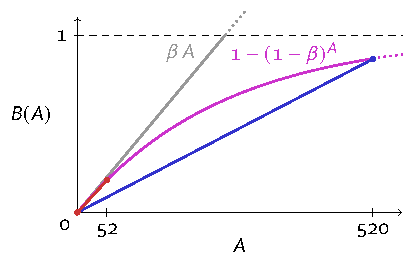
\includegraphics[scale=1]{binom.lin}}
      \caption{Models of probability of transmission:
        linear vs binomial and per-partnership vs per-partnership-year}
      \label{fig:binom.lin}
    \end{subfigure}\quad
    \begin{subfigure}[b]{0.55\widefig}
      \centerline{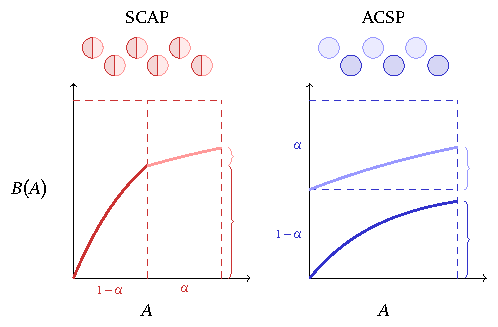
\includegraphics[scale=1]{binom.mod}}
      \caption{Transmission modifier affecting:
        some contacts in all partnerships vs all contacts in some partnerships}
      \label{fig:binom.mod}
  \end{subfigure}}
  \caption{Probability of transmission $B$ vs number of contacts (sex acts) $A$.
    (\subref{fig:binom.lin}) Illustrates linear (grey) vs binomial (purple) models for $B$,
    and compares the applied yearly \emph{rate} of transmission $QB$ (tangents)
    for $\delta = 1$ (red) vs $\delta = 10$ (blue) year partnership durations,
    with fixed contact frequency $F = 52$ per-year,
    and $\beta = 0.34\%$ from \cite{Boily2009}.
    (\subref{fig:binom.mod}) Compares interpretation of a transmission modifier
    with $R = 0.3$ effect and $\alpha = 0.5$ coverage as:
    some contacts in all partnerships (SCAP, red) from \eqref{eq:B.m.scap} vs
    all contacts in some partnerships (ACSP, blue) from \eqref{eq:B.m.acsp};
    sum of brace heights gives the modelled $B$.}
  \label{fig:binom}
\end{figure}
\paragraph{\case{1b} Binomial Per-Partnership-Year}
Many applications of model \case{1}
define the probability of transmission $B$ per-partnership-year,
and thus effectively choose partnership duration $\delta = 1$ year,
total contacts $A = F$ (yearly contact frequency per-partnership),
and partnership formation rate $Q \ge 1$,
even for long-duration partnerships.
We denote the model allowing $\delta > 1$ as \case{1a}
and that with $\delta = 1$ as \case{1b}, which appears to be more common.
As the ``true'' values of $\delta$, $F$, and/or $\beta$ increase,
model \case{1b} can be substantially different from \case{1a}. % as explored in \sref{sup.bin}.
Figure~\ref{fig:binom.lin} further illustrates two tangents,
whose slope represents the applied yearly transmission rate $QB$ for
$\delta = 1$ (red) vs $10$ (blue) year partnership durations,
with $\beta = 0.34\%$~\cite{Boily2009} and contact frequency $F = 52$ per-year.
The yearly transmission rate for $\delta = 1$ is nearly double the rate for $\delta = 10$,
and the binomial adjustment has almost no effect over 1 year:
$B(A\mid\delta=1) \approx \beta A$.
\paragraph{Transmission Modifiers}
Factors that alter the probability of infection,
such as condom use, circumcision, and STI co-infection,
are usually added to \eqref{eq:B} assuming
a relative probability $R$ and constant proportion of contacts affected $\alpha$.
For multiple modifiers, $B$ is often defined as:
\begin{equation}\label{eq:B.m.scap}
  B = 1 - \prod_{m} {(1 - R_m \beta)}^{\alpha_m\,A}
\end{equation}
where: $\sum_m \alpha_m = 1$;
some $R_m$ may represent the product of multiple factors;
and a dummy term $R_m = 1$ can apply to the proportion of contacts without any modifier.
In \eqref{eq:B.m.scap},
factors are modelled as ``some contacts in all partnerships'' (SCAP),
\emph{not} ``all contacts in some partnerships'' (ACSP).
% JK: alternate, more concrete example:
%``$\alpha_m = 50\%$ condom use'' is modelled as
%50\% of contacts in all partnerships protected by a condom,
%\emph{not} all contacts in 50\% of partnerships protected by a condom.
To model ASCP, $B$ may be defined instead as:
\begin{equation}\label{eq:B.m.acsp}
  B = \sum_{m} \alpha_m \left(1 - {(1 - R_m \beta)}^A\right)
\end{equation}
which is effectively a weighted average.
It can be shown that SCAP~\eqref{eq:B.m.scap} $\ge$ ACSP~\eqref{eq:B.m.acsp},
because any large probability of transmission
has disproportionate influence on \eqref{eq:B.m.scap},
even for a small proportion of contacts affected ($\alpha$ or $1-\alpha$),
whereas this influence is bounded by $\alpha$ or $1-\alpha$ in \eqref{eq:B.m.acsp},
as shown in Figure~\ref{fig:binom.mod}.
Figure~\ref{fig:B.mod.sens} explores the conditions under which
differences between SCAP and ACSP are greatest.
These conditions can be summarized as:
when $R < 1$, $0.5 < \alpha < 1$, and $A$ is large; or
when $R > 1$, $0 < \alpha < 0.5$, and $A$ is large, but not too large.
Although differences rarely exceeded 20\% in our analyses,
the more appropriate equation should likely be selected based on a factor's interpretation.
\paragraph{\case{2} Binomial Time Interval}
Another model for the force of infection
further generalizes the idea of escaping infection to consider
risk from all partnerships simultaneously:
\begin{equation}\label{eq:foi.2a}
  \lambda_i^{\case{2}}(\Delta_t) =
  1 - \prod_{k}\left(1 - \sum_{jh} \left(1 -
  {\left(1 - \beta_{hk}\right)}^{Q_{ijk} A_k \Delta_t}\right) \frac{I_{jh}(t)}{N_j}\right)
\end{equation}
which is technically a probability $\le 1$, not a rate as in \case{1}.
A simple version of this model was introduced in \cite{Auvert1990},
where the dependence on time period $\Delta_t$ was explicitly noted.
In principle, this model is more precise than \case{1},
provided that $\Delta_t$ is matched to the timestep of the numerical solver.
However, and the added precision may be insignificant as $\Delta_t$ is usually small.
Moreover, much like \case{1}, subsequent adaptations of this model have
used a period of $\Delta_t = 1$~year,
and then applied the resulting $\lambda_i$ as a rate over smaller timesteps.%
\footnote{One possible reason that $\Delta_t$ in \eqref{eq:foi.2a}
  has not been used correctly could be that:
  most numerical solvers for systems of ordinary differential equations
  pass only $t$ (not $\Delta_t$) to the derivative computing function,
  and may use adaptive $\Delta_t$ for precision while solving --- including:
  \texttt{scipy.integrate.odeint} in Python,
  \texttt{deSolve::lsoda} in R, and
  \texttt{ode45} in MATLAB.}
This adaptation then reduces transmission vs \case{1b},
since all contacts across all partnership-years
are considered in one binomial model.
\par
In \eqref{eq:foi.2a}, the prevalence of infection $I_{jh}/N_j$ is modelled as ACSP, not SCAP,
% JK: not sure whether the phrasing below helps or is just confusing.
reflecting ``homogeneous'' partnerships with a heterogeneous pool of partners, rather than
``heterogeneous'' partnerships with a homogeneous pool of partners.
As with transmission modifiers, this distinction is often ignored,
and using SCAP allows the following simplification of \eqref{eq:foi.2a}:%
%\footnote{Since multiplication/exponentiation of many small numbers is
%  computationally expensive and unstable,
%  it may be useful to solve \eqref{eq:foi.2b} and similar equations
%  using the ``exp-sum-log'' trick.}
\begin{equation}\label{eq:foi.2bi}
  \lambda_i^{\case{2}}(\Delta_t) =
  1 - \prod_{jhk}{\left(1 - \beta_{hk}\right)}^{Q_{ijk} A_k \Delta_t \frac{I_{jh}(t)}{N_j}}
\end{equation}
A further adaptation of \eqref{eq:foi.2bi} first computes
a weighted average per-contact transmission probability $\beta_{hk}$
given the prevalence of each infection stage among partners:
\begin{equation}\label{eq:foi.2b}
  \lambda_i^{\case{2}}(\Delta_t) =
  1 - \prod_{hk}{\left(1 - \sum_j \beta_{hk}\frac{I_{jh}(t)}{N_j}\right)}^{Q_{ijk} A_k \Delta_t}
\end{equation}
which often yields almost identical results to \eqref{eq:foi.2bi}
($<1\%$ difference in our exploration).
We refer to the ACSP model in \eqref{eq:foi.2a} as \case{2a},
and the SCAP model in \eqref{eq:foi.2b} as \case{2b}.
We have not seen \case{2a} used in the literature.
\paragraph{\case{3} Pure Rate}
As shown in Figure~\ref{fig:binom.lin}, the binomial adjustment in models \case{1-2}
has negligible effect when $\beta$, $A$, and/or $\Delta_t$ are sufficiently small,
at which point $B(A) \approx \beta A$.
For completeness, and since it will be useful later,
we define a final model \case{3} with exactly $B(A) = \beta A$:
\begin{equation}\label{eq:foi.3}
  \lambda_i^{\case{3}}(t) = \sum_{jhk} Q_{ijk} A_k \beta_{hk} \frac{I_{jh}(t)}{N_j}
\end{equation}
which effectively ignores partnership duration $\delta$.
\par
We further introduce an alternate parameterization to $QA$.
Whereas $QA$ reflects the partnership formation \emph{rate} $Q$
and \emph{number} of contacts per-partnership $A$,
we introduce $CF$, reflecting the \emph{number} of concurrent partnerships $C$
and contact \emph{frequency} per-partnership $F$.
For a given partnership duration $\delta$, we have $F = A/\delta$, and $C = \delta Q$;
thus, the total contact rate in both parameterizations is the same: $QA = CF$.
\paragraph{Limitations of Models \case{1-3}}
% TODO: update this given issues in how QA may be interpreted (!)
Models \case{1-3} span a continuum of trade-offs.
At one extreme, model \case{1a} appropriately reduces the proportion of infections
transmitted via long-duration partnerships;
however, in doing so, the reduced rate of transmission $QB$
effectively \emph{delays} transmission in such partnerships.
At the other extreme, model \case{3} ignores partnership duration,
and thus likely overestimates the proportion of infections
transmitted via long-duration partnerships;
however, no transmission is delayed by binomial adjustment.
In the middle, models \case{1b}, \case{2a}, and \case{2b} include
a small reduction in proportion of transmission via long-duration partnerships
and a small delay in transmission.
Furthermore, as noted above,
applying model \case{2} as a rate over smaller timesteps but using $\Delta_t = 1$
can substantially underestimate incidence among higher risk groups,
due to the probability constraint: (\ref{eq:foi.2a}--\ref{eq:foi.2b}) $\le$ 1.
\par
A final and critical limitation affecting all models \case{1-3}
is that partnerships are ``instantaneous''.
As such, newly infected individuals may immediately transmit infection
in the same partnership by which they were infected --- to an evidently already infected partner.
This transmission is possible because, with instantaneous partnerships,
the infection status of partners is averaged across the pool of available partners,
so a ``fraction'' of even one single partner is always susceptible (Figure~\ref{fig:tx.freq}).
In other words, incidence is always proportional to prevalence.
In reality, infections transmitted via long-duration partnerships become ``trapped'',
unless individuals have additional partners, or the partnership ends.
%\footnote{Some authors have described contacts following transmission within a given partnership
%  as ``wasted'' contacts.}
Thus, prevalence immediately increases,
but incidence may not increase proportionally until some time later, or ever.
